\documentclass{article}

%\usepackage{geometry}
\usepackage{graphicx}
\usepackage{amsmath}
\usepackage{hyperref}
\usepackage{float}


\title{LE3: Arrays vs Linked List}
\author{Kevin Lei}
\date{February 25, 2024}

\begin{document}

\maketitle

\section{Introduction}
In this lab exercise, we discuss the concept of caches and how they affect the performance of data structures. 
We will compare the performance of the \texttt{push} operation for a linked list and vector in C++ using data gathered with the \texttt{chrono} library.
Finally, we will apply the concepts of caching and access patterns to analyze the experimental results.

\section{Experimental Results}
The following graph shows the time taken to perform the \texttt{push} operation on a linked list and vector of size $n$.
\begin{figure}[H]
    \centering
    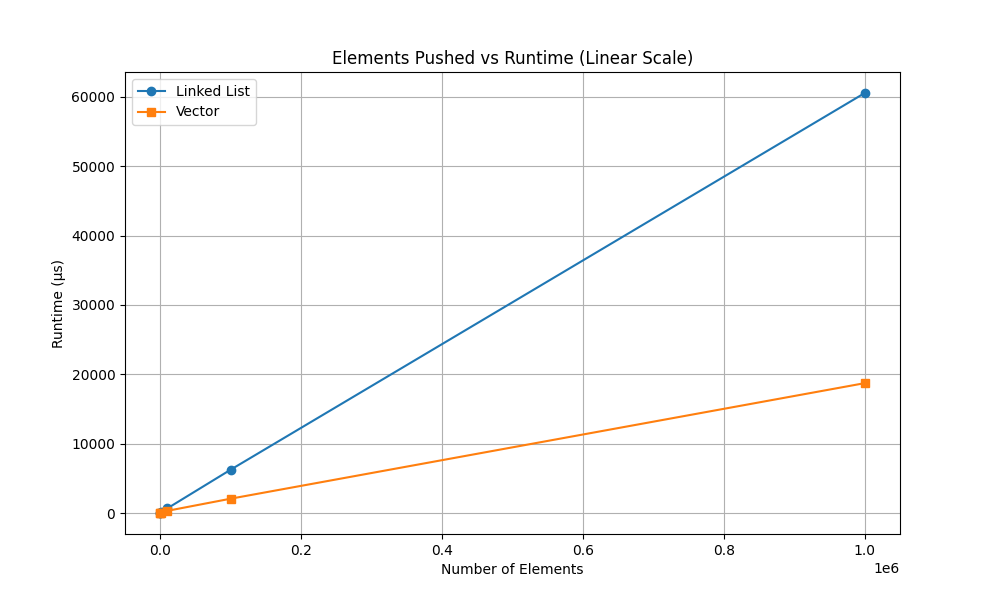
\includegraphics[width=\textwidth]{./images/linear.png}
    \caption{Runtime vs input size for linked list and vector.}
\end{figure}

\section{Analysis}
In theory, the \texttt{push} operation for both the linked list and vector should have an amortized time complexity of $O(1)$.
The linked list just needs to allocate a new node and update the pointers, and typically, the vector will just have to insert the new element at the end of the existing data.
Even though in the worst case the vector may have to reallocate and copy the entire array, the amortized time complexity is still $O(1)$.
This is consistent with our experimental results as shown above, however, we notice that the vector is consistently faster than the linked list.

The superior performance of the vector can be attributed to factors such as caching and memory access patterns. 
Arrays (vectors) use contiguous memory allocation, which enhances cache efficiency due to \textit{spatial locality}. 
This means that when an element of the array is used by the program, subsequent elements are likely already in the cache or will be fetched together, which reduces the need for frequent memory accesses. 
This advantage is particularly significant for operations like \texttt{push}, where elements are added sequentially, allowing processors to prefetch data effectively.
On the other hand, linked lists suffer from non-contiguous memory allocation. 
Each node may be allocated in a completely different memory location, leading to worse cache utilization. 
Since every node access has a higher chance of a cache miss, the performance impact becomes noticeable as the size of the data structure grows, which is what we observe in the graph.

We can see evidence that spacial locality is a significant factor in the performance of the \texttt{push} operation by observing the cachegrind output for the linked list and vector.
The linked list has a $0.2\%$ LLd cache miss rate, which is basically double the $0.1\%$ rate for the vector.
This is consistent with our theory that the vector has better cache efficiency due to spacial locality.

\end{document}
